\documentclass[11pt,a4paper]{article}
\usepackage{ngerman}
\usepackage[ngerman]{babel}
\usepackage[utf8x]{inputenc}
\usepackage[T1]{fontenc}
\usepackage{lmodern}
\usepackage{marvosym}
\usepackage{amsfonts,amsmath,amssymb}
\usepackage{textcomp}
\usepackage{pifont}
\usepackage{ifpdf}
\usepackage[pdftex]{color}
\ifpdf
  \usepackage[pdftex]{graphicx}
\else
  \usepackage[dvips]{graphicx}\fi

\pagestyle{empty}

\usepackage[scale=0.775]{geometry}
\setlength{\parindent}{0pt}
\addtolength{\parskip}{6pt}

\def\firstname{Pascal}
\def\familyname{Bernhard}
\def\FileAuthor{\firstname~\familyname}
\def\FileTitle{\firstname~\familyname's Salz}
\def\FileSubject{Salz}
\def\FileKeyWords{\firstname~\familyname, Salz}

\renewcommand{\ttdefault}{pcr}
\hyphenation{ins-be-son-de-re}
\usepackage{url}
\urlstyle{tt}
\ifpdf
  \usepackage[pdftex,pdfborder=0,breaklinks,baseurl=http://,pdfpagemode=None,pdfstartview=XYZ,pdfstartpage=1]{hyperref}
  \hypersetup{
    pdfauthor   = \FileAuthor,%
    pdftitle    = \FileTitle,%
    pdfsubject  = \FileSubject,%
    pdfkeywords = \FileKeyWords,%
    pdfcreator  = \LaTeX,%
    pdfproducer = \LaTeX}
\else
  \usepackage[dvips]{hyperref}
\fi

\definecolor{firstnamecolor}{RGB}{56,115,179}
\definecolor{familynamecolor}{RGB}{56,115,179}
\hypersetup{pdfborder=0 0 0}

% Gleiche Schriftart für Hyperlinks
\urlstyle{same}


%  Gefrickel um URL-Links vernünftig umzubrechen
\makeatletter
\g@addto@macro\UrlBreaks{
  \do\a\do\b\do\c\do\d\do\e\do\f\do\g\do\h\do\i\do\j
  \do\k\do\l\do\m\do\n\do\o\do\p\do\q\do\r\do\s\do\t
  \do\u\do\v\do\w\do\x\do\y\do\z\do\&\do\1\do\2\do\3
  \do\4\do\5\do\6\do\7\do\8\do\9\do\0}
% \def\do@url@hyp{\do\-}

% Hiermit soll einer übervolle Box verhindert werden -- funktioniert sogar irgendwie
\g@addto@macro\UrlSpecials{\do\/{\mbox{\UrlFont/}\hskip 0pt plus 1pt}}
\makeatother

% Farben werden hier definiert
\definecolor{MidnightBlue}{RGB}{0,103,149}


\begin{document}
\sffamily   % for use with a résumé using sans serif fonts;
%\rmfamily  % for use with a résumé using serif fonts;
\hfill%
\begin{minipage}[t]{.6\textwidth}
\raggedleft%
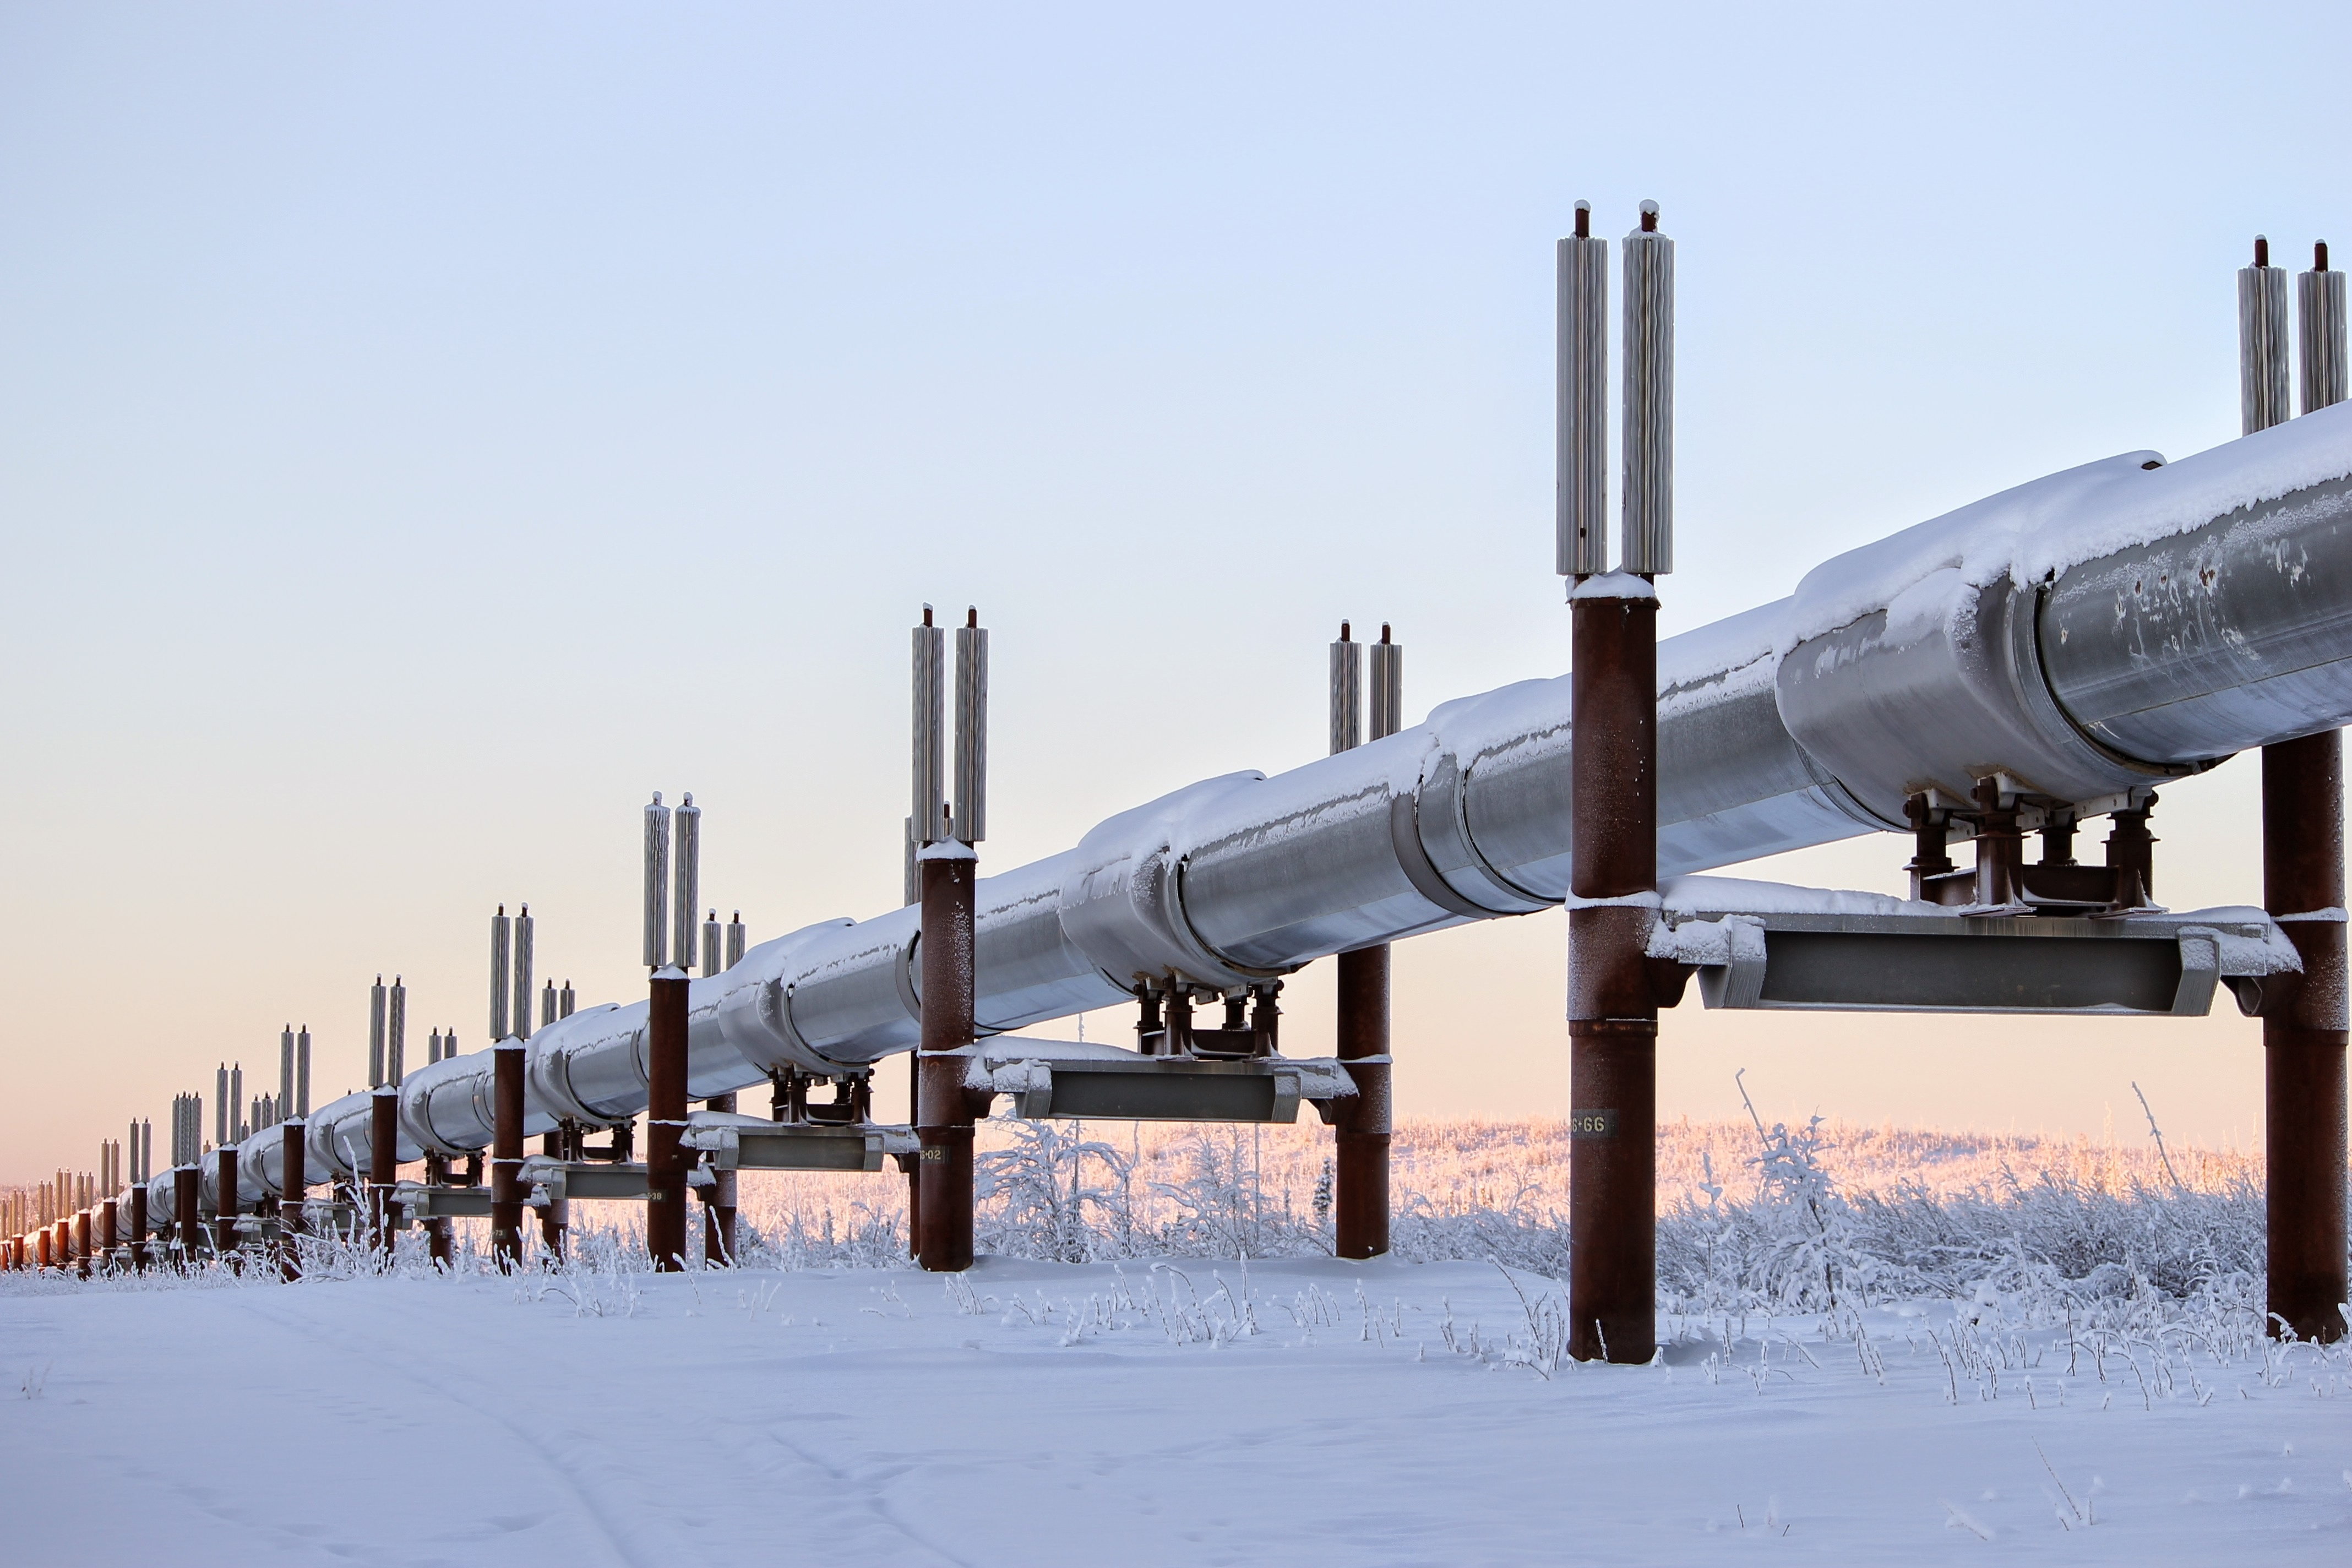
\includegraphics[width=0.55\textwidth]{Pipeline.jpg}


\end{minipage}\\[0.5em]
%
{\color{firstnamecolor}\rule{\textwidth}{.25ex}}
%
\begin{minipage}[t]{.4\textwidth}
	\raggedright%
	% {\bfseries {\color{firstnamecolor}
	\vspace*{1em}

	\small%
\end{minipage}
%
\hfill
%
\begin{minipage}[t]{.4\textwidth}
	\raggedleft % US style
	\today
	%April 6, 2006 % US informal style
	%05/04/2006 % UK formal style
\end{minipage}\\[2.2em]


{\bfseries \color{familynamecolor}{{\LARGE Energiepolitik im Baltikum -- Beispiel Erdgassektor}}}\\[0.75em]

\section*{\textsf{Besondere Eigenschaften von Gasmärkten}}

\begin{itemize}
\item der Gassektor kann in die drei Segmente \textbf{Upstream} -- \textbf{Midstream} -- \textbf{Downstream} gegliedert werden

	\begin{itemize}
	\item \textbf{Upstream:} Exploration von Lagerstätten und Förderung von Erdgas\\
	\ding{225} sehr kostenintensive Tätigkeiten, die mit erheblichen unternehmerischen Risiken verbunden sind\\
	\ding{225} geographisch gebundene Geschäftsaktivität, die meist in einem Spannungsverhältnis mit Souveränitätsansprüchen von Nationalstaaten steht (meist sind Staatsunternehmen in diesem Bereich tätig: \textsl{Gazprom})\\
	\ding{225} private Förderunternehmen müssen beträchtliche 'Royalties' an Staaten zahlen

	\vspace{1cm}

	\item \textbf{Midstream:} Transport von Erdgas mittels Pipelines oder auf Schiffen in Form von Flüssiggas\\
	\ding{225} natürliche Monopole im Bereich der Infrastruktur

	\vspace{1cm}

	\item \textbf{Downstream:} Endverteilung, bzw. Vertrieb von Erdgas and Endverbraucher (Haushalte und Unternehmen)

	\vspace{1cm}

	\end{itemize}

\item beträchtliche \textbf{Sunk Costs} für Exploration Förderung und Transport von Erdgas\\
\ding{225} Föderanlagen und Pipelines können nach dem Bau nicht einfach versetzt werden\\
\ding{225} Sunk Costs können später nicht oder nur zu einem geringem Teil zurückgewonnen werden\\

\item \textbf{natürliche Monopole} im Midstream-Bereich:\\
\ding{225} hohe Sunk Costs, erhebliche Skalenerträge, hohe Markteintrittsbarrieren (\textsl{sehr hohe fixe Kosten im Verhältnis zu den variablen Kosten})\\
\ding{225} es macht wirtschaftlich nur Sinn, wenn ein Unternehmen die Infrastruktur für die Fernleitung von Erdgas bereitstellt und betreibt\\
\ding{225} diese Monopolsituation gibt dem Infrastrukturbetreiber erhebliche Marktmacht und somit politischen Einfluss


\item in Europa haben sich traditionell auf Gasmärkten sog. \textbf{vertikal integrierte Unternehmen} herausgebildet\\
\ding{225} da Energieversorgung meist als öffentliches Gut erachtet wurde, zumeist staatliche Monopolisten


\end{itemize}




\subsection*{\textsf{Gasmärkte in den baltischen Ländern}}

\begin{itemize}

\item Estland, Lettland \& Litauen besitzen selbst keine nennenswerten Vorkommen an fossilen Brennträgern\\
\ding{225} Primärenergie muss aus dem Ausland importiert werden
\ding{225} Baltikum ist eine \textbf{Energieinsel}

\item bis Anfang 2015 waren die baltischen Ländern gänzlich auf russisches Erdgas angewiesen, da keine Pipelines zu europäischen Gasnetzen bestehen

\item \textsl{Gazprom} hält an den staatlichen Energieversorgern \emph{Lietuvos dujos} und \emph{Lativjas G\={a}ze} große Anteile mit Kontrollmacht\\
\ding{225} Vize-Präsident von \emph{Lativjas G\={a}ze} Juris Savickis ist Ex-KGB Agent\\
\ding{225} politisch brisante Kombination aus Monopolsituation der Gasunternehmen und russischem Einfluss auf den baltischen Gasmärkten\\
\ding{225} der westliche Anteilseigner an \emph{Lietuvos dujos} und \emph{Lativjas G\={a}ze} ist die \textsl{E.ON Ruhrgas AG}, die traditionell gute Beziehungen zu ihren russischen Geschäftspartnern unterhält und Interesse an enger Kooperation mit Russland hat

\end{itemize}



\subsection*{\textsf{Salz im Mittelalter Europas}}



\subsection*{\textsf{Neuzeit}}



\end{document}